In MMseqs, the prefiltering stage is the first step to process all sequences and serves to reduce the search space significantly, therefore it's imperative for the algorithm to be as efficient as possible. Query sequences are searched one by one against the target set (Fig. 1b, loop 1). For each k-mer starting position in the query (loop 2) we generate a list of all similar k-mers (orange frame) with a Blosum62 similarity above a threshold score. Lower threshold scores (option --k-score) result in higher average numbers of similar k-mers and thereby higher sensitivity and lower speed. The similar k-mers are generated with a linear-time branch-and-bound algorithm. For each k-mer in the list of similar k-mers (loop 3), we obtain from the index table (blue frame) the list of target sequence identifiers targetID and the positions j of the k-mer (green frame). In the last step the corresponding score in the target score vector is incremented.

\begin{center}
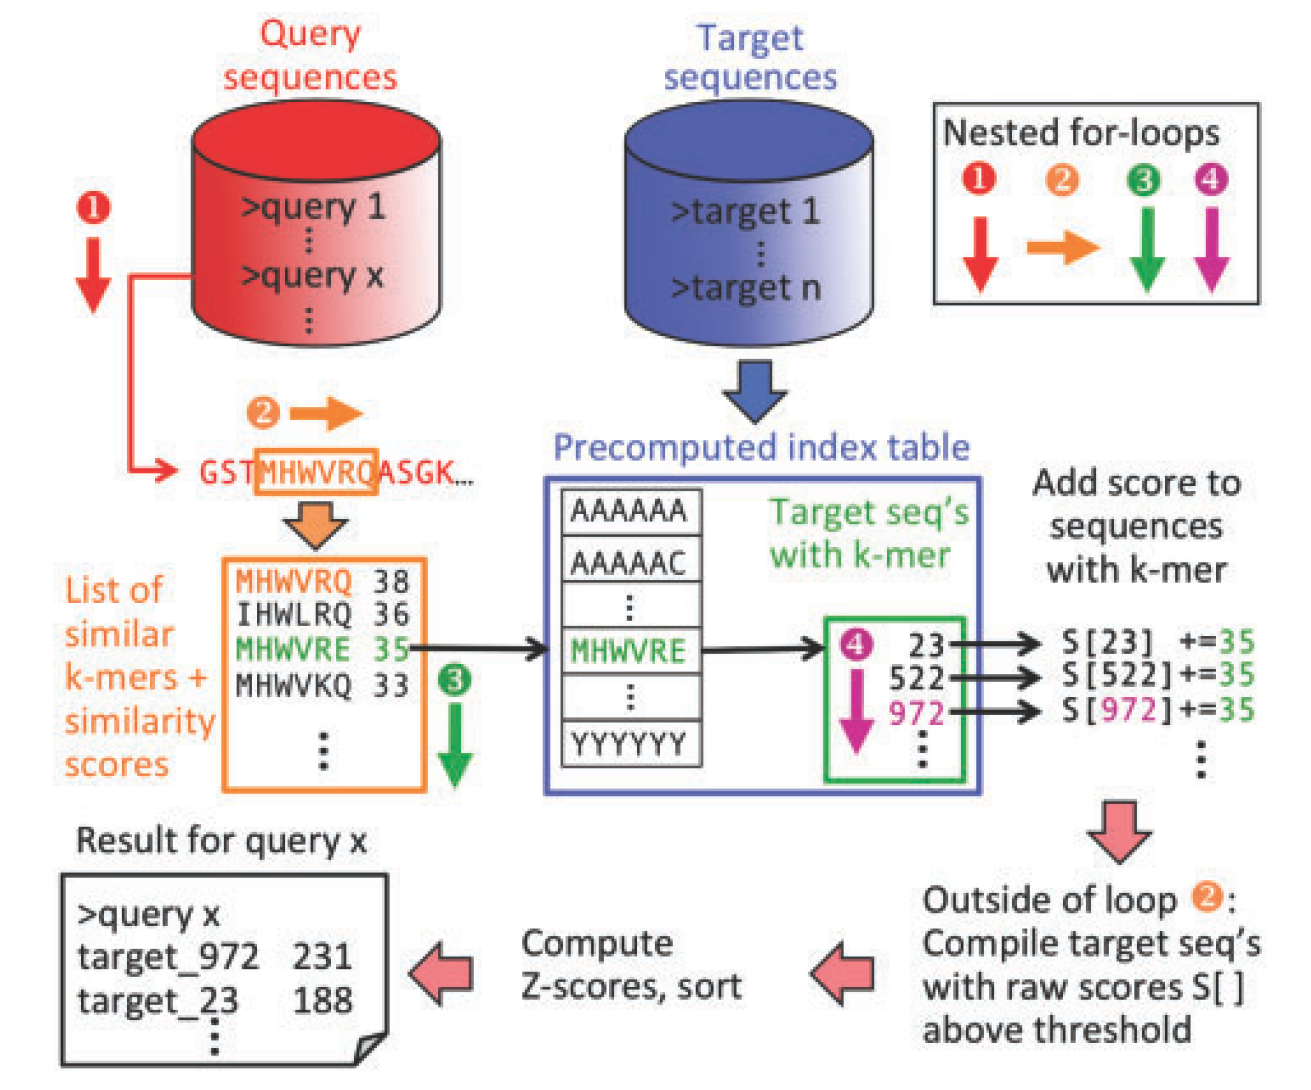
\includegraphics[scale=0.3]{graphics/MMseqs_prefilter.png}
\end{center}

In MMseqs2, the prefiltering stage was reengineered. In the innermost loop 4 we go through this list to detect double k-mer matches by comparing the current diagonal ij with the previously matched diagonal for targetID. If the previous and current diagonals agree, we store the diagonal i-j and targetID as a double match.

\begin{center}
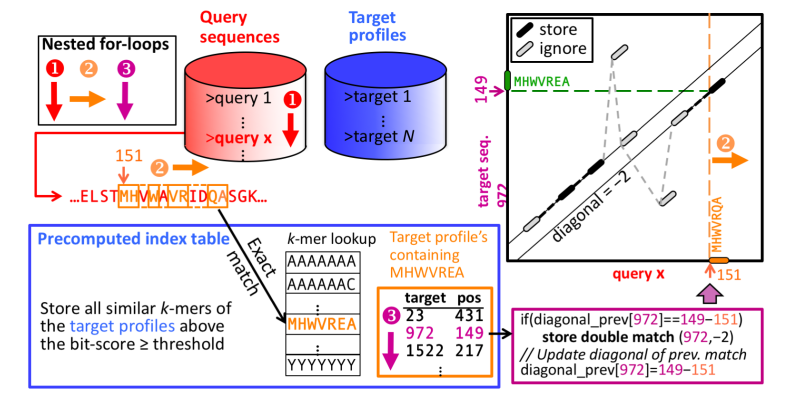
\includegraphics[scale=0.5]{graphics/MMseqs2_prefilter.png}
\end{center}
